\documentclass{beamer}
%\documentclass[handout]{beamer}
% This file is a solution template for:

% - Giving a talk on some subject.
% - The talk is between 15min and 45min long.
% - Style is ornate.

% Copyright 2004 by Till Tantau <tantau@users.sourceforge.net>.
%
% In principle, this file can be redistributed and/or modified under
% the terms of the GNU Public License, version 2.
%
% However, this file is supposed to be a template to be modified
% for your own needs. For this reason, if you use this file as a
% template and not specifically distribute it as part of a another
% package/program, I grant the extra permission to freely copy and
% modify this file as you see fit and even to delete this copyright
% notice. 


\mode<presentation>
{
  \usetheme{Montpellier}

  %\setbeamercovered{transparent}
  % or whatever (possibly just delete it)
}

\usepackage{xmpmulti} % package that defines \multiinclude

\usepackage[english]{babel}

\usepackage[latin1]{inputenc}

\usepackage{times}
\usepackage[T1]{fontenc}
% Or whatever. Note that the encoding and the font should match. If T1
% does not look nice, try deleting the line with the fontenc.

%\title [short title] (optional, use only with long paper titles)
\title{Sleeping experts \\ and \\ Expert Engineering}

\author[Freund] % (optional, use only with lots of authors)
{Yoav Freund}
% - Give the names in the same order as the appear in the paper.
% - Use the \inst{?} command only if the authors have different
%   affiliation.

\institute[Universities of Somewhere and Elsewhere] % (optional, but mostly needed)

\subject{Machine Learning}
% This is only inserted into the PDF information catalog. Can be left
% out. 

% If you have a file called "university-logo-filename.xxx", where xxx
% is a graphic format that can be processed by latex or pdflatex,
% resp., then you can add a logo as follows:

% \pgfdeclareimage[height=0.5cm]{university-logo}{university-logo-filename}
% \logo{\pgfuseimage{university-logo}}



% Delete this, if you do not want the table of contents to pop up at
% the beginning of each subsection:
%% \AtBeginSubsection[]
%% {
%%   \begin{frame}<beamer>
%%     \frametitle{Outline}
%%     \tableofcontents[currentsection,currentsubsection]
%%   \end{frame}
%% }


% If you wish to uncover everything in a step-wise fashion, uncomment
% the following command: 

\beamerdefaultoverlayspecification{<+->}

\newcommand{\newmcommand}[2]{\newcommand{#1}{{\ifmmode {#2}\else\mbox{${#2}$}\fi}}}
\newcommand{\newmcommandi}[2]{\newcommand{#1}[1]{{\ifmmode {#2}\else\mbox{${#2}$}\fi}}}
\newcommand{\newmcommandii}[2]{\newcommand{#1}[2]{{\ifmmode {#2}\else\mbox{${#2}$}\fi}}}
\newcommand{\newmcommandiii}[2]{\newcommand{#1}[3]{{\ifmmode {#2}\else\mbox{${#2}$}\fi}}}

\newcommand{\algfnt}{\bf}

\newmcommand{\ouralg}{{\mbox{\algfnt Hedge}({\eta})}}

\newmcommand{\iter}{T}

\newfont{\cmmib}{cmmib10}
\newcommand{\boldell}{{\mbox{\cmmib \symbol{'140}}}}

\newmcommandi{\costvec}{{\boldell}^{#1}}
\newmcommandii{\cost}{{\ell}^{#1}_{#2}}

\newmcommandi{\rd}{\tilde{#1}}

\newmcommandi{\distvec}{{\bf p}^{#1}}
\newmcommandi{\rddistvec}{\rd{\bf p}^{#1}}
\newmcommandii{\dist}{{p}^{#1}_{#2}}
\newmcommandii{\rddist}{\rd{p}^{#1}_{#2}}

\newmcommandi{\bdistvec}{{\bf q}^{#1}}
\newmcommandii{\bdist}{{q}^{#1}_{#2}}

\newmcommandi{\wtvec}{{\bf w}^{#1}}
\newmcommandi{\rdwtvec}{\rd{\bf w}^{#1}}
\newmcommandii{\wt}{{w}^{#1}_{#2}}
\newmcommandii{\rdwt}{\rd{w}^{#1}_{#2}}

\newcommand{\w}[1]{\makebox[12pt]{{#1}}}
\newcommand{\Rps}{\mbox{\tt R}}
\newcommand{\rPs}{\mbox{\tt P}}
\newcommand{\rpS}{\mbox{\tt S}}
\newcommand{\rpstie}{\w{$\frac{1}{2}$}}
\newcommand{\rpswin}{\w{$0$}}
\newcommand{\rpsloss}{\w{$1$}}

\newmcommand{\decspace}{\Delta}
\newmcommand{\decsym}{\delta}
\newmcommandi{\dec}{\decsym^{#1}}
\newmcommand{\decdistsym}{\cal D}
\newmcommandi{\decdist}{{\decdistsym}^{#1}}

\newmcommand{\simpdistspace}{{\bf \cal S}}
\newmcommand{\domset}{{\rm dom}(\decdistsym)}

\newmcommand{\expdistsym}{{\cal E}}
\newmcommandii{\expdist}{{\expdistsym}^{#1}_{#2}}
\newmcommand{\expdecsym}{{\varepsilon}}
\newmcommandii{\expdec}{\expdecsym^{#1}_{#2}}

\newmcommand{\outspace}{\Omega}
\newmcommand{\outsym}{\omega}
\newmcommandi{\out}{\outsym^{#1}}

%\newmcommandii{\Dkl}{D_{\mbox{kl}}\paren{#1||#2}}
\newmcommandii{\Dkl}{{\rm {KL}}\paren{{#1}\;||\;{#2}}}

\newmcommandi{\sumwts}{\sum_{i=1}^N \wt{#1}{i}}

\newmcommand{\lossalg}{L_A}
\newmcommand{\lossouralg}{{L_{\mbox{\scriptsize\algfnt Hedge}(\eta)}}}
\newmcommand{\lossS}{{L_{\mbox{\scriptsize\algfnt S}}}}
\newmcommandi{\lossi}{L_{#1}}
\newmcommandii{\lossit}{L_{#1}^{#2}}

\newmcommandi{\upbnd}{\tilde{#1}}

\newcommand{\angles}[1]{{\left\langle {#1} \right\rangle}}
\newcommand{\paren}[1]{{\left( {#1} \right)}}
\newcommand{\abs}[1]{{\left| {#1} \right|}}
\newcommand{\ceiling}[1]{{\left\lceil {#1} \right\rceil}}

\newfont{\msym}{msbm10}
\newcommand{\real}{\mbox{\msym R}}

\newmcommand{\updatefcn}{U_\eta}

%% \newtheorem{theorem}{Theorem}	
%% \newtheorem{lemma}[theorem]{Lemma}
%% \newtheorem{corollary}[theorem]{Corollary}
%% \newtheorem{definition}{Definition}

%\newcommand{\proof}{\noindent{\bf Proof:} }
%\newcommand{\example}[1]{{\em Example #1.} }
%\newcommand{\qed}{\rule{0.7em}{0.7em}}

\newcommand{\WeakAlg}{\mbox{\algfnt WeakLearn}}
\newcommand{\Boost}{\mbox{\algfnt AdaBoost}}
\newcommand{\EX}{\mbox{\bf EX}}
\newmcommand{\hf}{h_{{f}}}
\newmcommand{\rdhf}{\rd{h}_{{f}}}
\newmcommand{\hfT}{h^T_{{f}}}
\newmcommand{\ranh}{{b}}

\newmcommand{\conclass}{{\cal C}}

\newmcommand{\badvec}{{\bf b}}
\newmcommandi{\bad}{{b}_{#1}}

%%%%%%%% New commands defined for the game-playing paper

\newmcommand{\hedge}{\algfnt Hedge}
\newmcommand{\play}{\algfnt Play}
\newmcommandi{\Glossvec}{{\bg y}^{#1}}
\newmcommandii{\Gloss}{{y}^{#1}_{#2}}
%\newmcommandi{\action}{{I}_{#1}}
\newmcommandi{\Gdistvec}{{\bf \tilde{p}}^{#1}}
\newmcommandii{\Gdist}{{\teilde{p}}^{#1}_{#2}}

%%%%%%%%%%%%%%%%%%%%%%%%%%%%%%%%%%%%%%%%%%%%%%%%%%%%%
\newmcommand{\Idistvec}{{D}}
\newmcommandi{\Idist}{\Idistvec({#1})}
\newmcommand{\Idistt}{\Idistvec_t}

\newmcommand{\Xdist}{{\cal P}}
\newmcommand{\emp}{\hat{\epsilon}}

\newmcommand{\classpc}{Y}
\newmcommand{\numclass}{k}
\newmcommandii{\prob}{\mbox{\rm Pr}_{#1}\left[{#2}\right]}
\newmcommandii{\exval}{\mbox{\rm E}_{#1}\left[{#2}\right]}

\newmcommand{\lab}{y}
\newmcommand{\ploss}{\mbox{ploss}}
\newmcommandii{\avploss}{\ploss_{#1}({#2})}
\newcommand{\sfrac}[2]{\mbox{$\frac{#1}{#2}$}}

\newcommand{\mboosta}{\mbox{\algfnt AdaBoost.M1}}
\newcommand{\mboostb}{\mbox{\algfnt AdaBoost.M2}}
\newcommand{\mboostr}{\mbox{\algfnt AdaBoost.R}}

\newmcommand{\slos}{\mbox{ploss}}
\newmcommandiii{\sloss}{\slos_{#1}({#2},{#3})}
\newmcommandiii{\avsloss}{\slos_{{#1},{#2}}({#3})}

\newmcommandii{\vwt}{{W}^{#1}_{#2}}

\newcommand{\figline}{\rule{\textwidth}{1pt}}

%\newmcommandi{\1}{{\bf 1}({#1})}
\newmcommandi{\1}{[\![{#1}]\!]}

\newmcommand{\confcn}{\kappa}
\newmcommandi{\erint}{\abs{\int_{y_i}^{h_t(x_i)} {#1} dy}}
%\newmcommandi{\erint}{\int_{\min\{y_i,h_t(x_i)\}}^{\max\{y_i,h_t(x_i)\}}{#1}dy}

\newcommand{\blue}[1]{{\color{blue}{#1}}}
\newcommand{\red}[1]{{\color{red}{#1}}}
\newcommand{\redEq}[1]{{\color{red}{$#1$}}}
\newcommand{\W}{\vec{W}}
\newcommand{\V}{\vec{V}}
\newcommand{\X}{\vec{X}}
\newcommand{\loss}{\vec{\ell}}
\newcommand{\HedgeLoss}{L_{\mbox{\footnotesize Hedge}}}

%%%%%%%%%%%%%%%%%%%%%%%%%%%%%%%%%%%%%%%%%%%%%%%%%%%%%%%%%%%%%%%%%%%%%%%%%%%%
%                                 MACROS                                   %
%%%%%%%%%%%%%%%%%%%%%%%%%%%%%%%%%%%%%%%%%%%%%%%%%%%%%%%%%%%%%%%%%%%%%%%%%%%%

%% \newcommand{\nats}{\mbox{\msym N}}

%% \newmcommand{\predspace}{\Phi}

\newmcommandii{\advice}{x_{{#2},{#1}}}
\newmcommandi{\advicei}{x_{#1}}
\newmcommandi{\advicevec}{{\bf x}_{#1}}
\newmcommandi{\pred}{\hat{y}_{#1}}
\newmcommandi{\outcome}{y_{#1}}

\newmcommandii{\sloss}{\ell_{#1}^{#2}}
\newmcommandi{\algloss}{\ell_A^{#1}}
\newmcommand{\talgloss}{L_A}

%%\newmcommand{\vu}{{\bf u}}	% the optimal weighting of the specialists
%%\newmcommand{\vv}{{\bf v}}
\newmcommandi{\uu}{u_{#1}}

\newmcommandi{\vp}{{\bf p}_{#1}} % the $t$th distribution chosen by
				 % the algorithm
\newmcommandii{\pp}{p_{{#2},{#1}}}
%%\newmcommandi{\ppi}{p_{#1}}	% an element of \vp at an unspeciafied
				% time
\newmcommand{\Bayes}{{\bf Bayes}} % Bayes algorithm
\newmcommand{\SBayes}{{\bf SBayes}} % Bayes algorithm for Specialists
%% \newmcommand{\SAbs}{{\bf SAbs}}	%Absolute loss algorithm with experts

%% \newmcommand{\SI}{{\bf WMS}}
%% \newmcommand{\SII}{{\bf EGS}}
%% \newmcommandii{\RE}{{\mbox{\bf RE} \left( #1 \| #2 \right)}}
%% \newmcommand{\updatefcn}{U_\beta}

%% \newcommand{\ohone}{\{0,1\}}
%% \newcommand{\luf}{\mu}
%% \newcommand{\angles}[1]{\left\langle {#1} \right\rangle}
% Rob's new macros
\newmcommand{\pfunc}{{\rm pred}}
\newmcommand{\pfuncN}{\pfunc_N}
\newmcommand{\ufunc}{{\rm update}}
\newmcommand{\ufuncN}{\ufunc_N}
\newmcommandi{\simplex}{\Delta_{#1}}
\newmcommandi{\aset}{{E_{#1}}}
\newmcommandi{\resadvicevec}{\advicevec{#1}^\aset{#1}}
\newmcommandii{\resadvice}{\advice{#1}{#2}^\aset{#2}}
\newmcommandi{\resadvicei}{\advicei{#1}^\aset{}}
\newmcommandii{\rvpp}{\vp{#1}^\aset{#2}}
%\newcommand{\rvpp}[2]{{\bf p}_{#1}^\aset{#2}}
\newmcommandi{\rvp}{\rvpp{#1}{#1}}
\newmcommandii{\rpp}{\pp{#1}{#2}^\aset{#2}}
\newmcommandi{\rppi}{\ppi{#1}^\aset{}}
\newmcommandi{\rvu}{\vu^\aset{#1}}
\newmcommand{\EG}{{\bf EG}}
\newmcommand{\SEG}{{\bf SEG}}
\newmcommandi{\closs}{\loss_{#1}}
\newmcommandi{\clossi}{\loss_{#1}^{I}}
\newmcommandi{\clossii}{\loss_{#1}^{II}}
\newmcommandi{\clossiii}{\loss_{#1}^{I/II}}
%%\newmcommandi{\paren}{\left({#1}\right)}

\newcommand{\cpred}{b}
\newcommand{\String}{s}
\newcommand{\uptok}{\ohone^{\le k}}
\newmcommand{\pgraph}{\cal G}
\newmcommand{\prun}{\cal P}
\newmcommand{\ginst}{z^t}
\newmcommand{\prior}{p_{1}}
\newmcommand{\pdist}{\nu}
\newmcommandii{\swp}{p^{#1}_{#2}}
\newmcommandii{\sswp}{Q^{#2}_{#1}}
\newmcommandi{\sumf}{F_{#1}}
\newmcommandii{\sfac}{R^{#2}_{#1}}
\newmcommand{\partexp}{S}

%%%%%%%%%%%%%%%%%%%%%%%%%%%%%%%%%%%%%%%%%%%%%%%%%%%%%%%%%%%%%%%%%%%%%%%%%%%%
%                              END OF MACROS                               %
%%%%%%%%%%%%%%%%%%%%%%%%%%%%%%%%%%%%%%%%%%%%%%%%%%%%%%%%%%%%%%%%%%%%%%%%%%%%

\begin{document}

%\iffalse %%%%%%%%%%%%%%%%%%%%%%%%%%%%%%%%%%%%%%%%%%%%%%%%%%%%%%%%%%%%%%%%%%

\begin{frame}
  \titlepage
\end{frame}

\begin{frame}
  \frametitle{Outline}
  \tableofcontents[pausesections]
  % You might wish to add the option [pausesections]
\end{frame}


\section{Sleeping Experts}

\begin{frame}
\frametitle{Specialists}
\begin{itemize}
\item Also called sleeping experts
\item The basic idea: specialists can associate a {\em confidence} with
  their predictions.
\item Master's prediction depends more on the confident predictions.
\item The weight of confident experts is changed more than that of
  unconfident ones.
\end{itemize}
\end{frame}

\begin{frame}
\frametitle{The specialists protocol}

\begin{enumerate}
\item
The adversary chooses a set \R{$\aset{t} \subseteq \{1,\ldots,N\}$} of
specialists that are awake at iteration \R{$t$}.
\item
The adversary chooses a prediction \R{$\advice{i}{t}$} for each awake
specialist \R{$i \in \aset{t}$}. 
\item
The algorithm chooses its own prediction \R{$\pred{t}$}.
\item
The adversary chooses an outcome \R{$\outcome{t}$}.
\item
The algorithm suffers loss \R{$\algloss{t} = \loss(\pred{t},\outcome{t})$}
and each of the awake specialists suffers loss 
\R{$\sloss{i}{t}=\loss(\advice{i}{t},\outcome{t})$}. 
Specialists that are asleep suffer no loss.
\end{enumerate}
\end{frame}

\subsection{Log Loss}

\begin{frame}
\frametitle{Log Loss}
\begin{itemize}
\item Log loss is the simplest case
\item
\R{\[
\loss(\pred{},\outcome{}) =
  \begin{cases}
          - \ln \pred{}
        & if $\outcome{} = 1$ \cr
           - \ln (1-\pred{})
        & if $\outcome{} = 0$.
  \end{cases}
\]}
\end{itemize}
\end{frame}

\begin{frame}
\frametitle{The standard Bayes algorithm (normalized weights)}
{\noindent {\bf Do for}} \R{$t=1,2,\ldots,T$}
\begin{enumerate}
 \item Predict with the weighted average of the experts
predictions:\newline
  \R{$$
	\pred{t} = \sum_{i=1}^N \pp{i}{t} \advice{i}{t} 
  $$}
 \item Observe outcome \R{$\outcome{t}$}
 \item Calculate a new posterior distribution:
\R{\[
\pp{i}{t+1} = 
\begin{cases}
            \frac{{\displaystyle \pp{i}{t} \advice{i}{t}}
             }{
             {\displaystyle \pred{t}}}
        & if $\outcome{t}=1$ \cr
\frac{{\displaystyle \pp{i}{t} (1-\advice{i}{t})}}{
            {\displaystyle  1-\pred{t}}}
        & if $\outcome{t}=0$.
\end{cases}
\]}
\end{enumerate}
\end{frame}

\begin{frame}
\frametitle{Bayes for Specialists}
{\noindent {\bf Do for}} \R{$t=1,2,\ldots,T$}
\begin{enumerate}
 \item Predict with the weighted average of the predictions of the
awake specialists:
  \R{$$
	\pred{t} = \frac{ \sum_{i \in \aset{t}} \pp{i}{t} \advice{i}{t} 
                     }{ 
                     \sum_{i \in \aset{t}} \pp{i}{t} }
  $$}
 \item Observe outcome \R{$\outcome{t}$} 
 \item Calculate a new posterior distribution: \\
\B{If} \R{$i \in \aset{t}$} \B{then}
\R{\[
\pp{i}{t+1} = 
\begin{cases}
            \frac{{\displaystyle \pp{i}{t} \advice{i}{t}}
             }{
             {\displaystyle \pred{t}}}
        & if $\outcome{t}=1$ \cr
           \frac{{\displaystyle \pp{i}{t} (1-\advice{i}{t})}
             }{
            {\displaystyle  1-\pred{t}}}
        & if $\outcome{t}=0$.
\end{cases}
\]}
\B{Otherwise:} \R{$\pp{i}{t+1}=\pp{i}{t}$}
\end{enumerate}
\end{frame}

\begin{frame}
\frametitle{Bound on Bayes for Specialists}
\begin{theorem} \label{thm:SBayes}
For any sequence of 
awake specialists, specialist predictions and outcomes
and for any distribution \R{$\vu$} over \R{$\{1,\ldots, N\}$}, the loss of
\B{\SBayes} satisfies
\R{\[
 \sum_{t=1}^T u(\aset{t}) \loss(\pred{t},\outcome{t})
\leq
 \sum_{t=1}^T 
  \sum_{i \in \aset{t}} \uu{i} \loss(\advice{i}{t},\outcome{t})
+
  \RE{\vu}{\vp{1}}~.
\]}
Where \R{$$u(\aset{t})\doteq \sum_{i \in E_t}u_i$$}
\end{theorem}
\end{frame}

\begin{frame}
\frametitle{Proof of Theorm}
\begin{itemize}
\item for each step:
\R{\begin{eqnarray}
\lefteqn{\RE{\vu}{\vp{t}} - \RE{\vu}{\vp{t+1}}} \nonumber \\
&=&
u(\aset{t}) \loss(\pred{t},\outcome{t})
- \sum_{i \in \aset{t}} \uu{i} \loss(\advice{i}{t},\outcome{t}).
 \label{eqn:Bayes-pred}
\end{eqnarray}
}
\item Summing over \R{$t=1,\ldots,T$} and using that
relative entropy is always positive:
\R{
\begin{eqnarray*}
  \RE{\vu}{\vp{1}}
 \!\!\!\! & \geq & \!\!\!\!
     \RE{\vu}{\vp{1}} - \RE{\vu}{\vp{T+1}}  \\
 \!\!\!\! & = &    \!\!\!\!
\sum_{t=1}^T u(\aset{t}) \loss(\pred{t},\outcome{t})
       -  \sum_{t=1}^T \sum_{i\in\aset{t}} \uu{i} \loss(\advice{i}{t},\outcome{t}).
\end{eqnarray*}
}
\end{itemize}
\end{frame}

\subsection{General Loss}
\begin{frame}
\frametitle{Using general loss functions}
We focus on algorithms which, like \B{\Bayes}, maintain a
distribution vector \R{$\vp{t}\in \simplex{N}$}.
Such algorithms are defined by two functions:
\begin{enumerate}
\item
\R{$$\pfunc: \simplex{N}\times [0,1]^N \rightarrow [0,1]$$}
which maps the current weight vector \R{$\vp{t}$} and instance
\R{\advicevec{t}} to a prediction \R{\pred{t}}; and
\item
\R{$$\ufunc: \simplex{N}\times [0,1]^N\times [0,1] \rightarrow
  \simplex{N}$$}
which maps the current weight vector \R{$\vp{t}$}, instance
\R{\advicevec{t}} and outcome \R{\outcome{t}} to a new weight vector
\R{$\vp{t+1}$}
\end{enumerate}
\end{frame}

\begin{frame}
\frametitle{Generic Insomniac Algorithm}
{\noindent {\bf Do for}} \R{$t=1,2,\ldots,T$}
\begin{enumerate}
 \item Observe \R{\advicevec{t}}
 \item Predict \R{$\pred{t} = \pfunc(\vp{t},\advicevec{t})$}
 \item Observe outcome \R{$\outcome{t}$} and 
       suffer loss \R{$\loss(\pred{t},\outcome{t})$}
 \item Calculate the new weight vector\\
	 \R{$\vp{t+1} = \ufunc(\vp{t},\advicevec{t},\outcome{t})$}
\end{enumerate}
\end{frame}

\begin{frame}
\frametitle{Generic Specialist Algorithm}
{\noindent {\bf Do for}} \R{$t=1,2,\ldots,T$}
\begin{enumerate}
 \item Observe \R{\aset{t}} and \R{\resadvicevec{t}}.
 \item Predict \R{$\pred{t} = \pfunc(\rvp{t},\resadvicevec{t})$}
 \item Observe outcome \R{$\outcome{t}$} and 
       suffer loss \R{$\loss(\pred{t},\outcome{t})$}.
 \item Calculate the new weight vector
	 \R{$\vp{t+1}$} so that it satisfies the following:
   \begin{enumerate}
      \item \R{$\pp{i}{t+1} = \pp{i}{t}$ for $i\not\in \aset{t}$}
      \item \R{\mbox{$\rvpp{t+1}{t} = \frac{1}{z_t} \ufunc(\rvp{t},\resadvicevec{t},\outcome{t})$}}
      \item \R{$\sum_{i=1}^N \pp{i}{t+1} = 1$}
      \item or Equivalently: \R{$\sum_{i \in \aset{t}} \pp{i}{t+1} = \sum_{i \in \aset{t}} \pp{i}{t}$}
   \end{enumerate}
\end{enumerate}
\end{frame}

\begin{frame}
\frametitle{Comparison cumulative losses for specialists}
\begin{itemize}
\item Comparison to average loss.
\R{\[
\min_{\vu \in \simplex{N}} \sum_{t=1}^T 
\clossi{\vu}(\advicevec{t},\outcome{t}) 
\;\; \mbox{ where }\;\; 
\clossi{\vu}(\advicevec{t},\outcome{t}) \doteq
\frac{\sum_{i \in \aset{t}} u_i \; \loss(\advice{i}{t},\outcome{t})}{\sum_{i \in \aset{t}} u_i}~.
\]}
\item Comparison to average prediction.
\R{\[
\min_{\vu \in \simplex{N}} \sum_{t=1}^T 
\clossii{\vu}(\advicevec{t},\outcome{t})
\;\; \mbox{ where } \;\; 
\clossii{\vu}(\advicevec{t},\outcome{t}) \doteq
  \loss \left(
   \frac{\sum_{i \in \aset{t}} u_i \advice{i}{t}}
        {\sum_{i \in \aset{t}} u_i}
   ,\outcome{t}
  \right)
\]}

\end{itemize}
\end{frame}

\begin{frame}
\frametitle{Analysis using relative entropy}
\begin{itemize}
\item Log-Loss / Bayes
\R{\[
  \RE{\vu}{\vp{t}} - \RE{\vu}{\vp{t+1}}
    = \loss(\pred{t},\outcome{t})
       - \sum_{i=1}^N \uu{i} \loss(\advice{i}{t},\outcome{t}).
\]}
\item General Vovk-style algorithm:
\R{\begin{equation*} \label{eqn:core}
  c\paren{\RE{\vu}{\vp{t}} - \RE{\vu}{\vp{t+1}}}
    \geq \loss(\pred{t},\outcome{t})
       - a \closs{\vu}(\advicevec{t},\outcome{t}).
\end{equation*}
}
Where \R{$\closs{}$} is \R{$(a,c)$}-achievable (Using Vovk with \R{$\eta=a/c$})
\end{itemize}
\end{frame}

\begin{frame}
\frametitle{Bound for general loss sleeping experts}
For any achievable \R{$(a,c)$}
\R{\begin{eqnarray*} \label{eqn:sleepbound}
  \sum_{t=1}^T u(\aset{t})\loss(\pred{t},\outcome{t}) \leq
    a \sum_{t=1}^T u(\aset{t})\closs{\rvu{t}}(\resadvicevec{t},\outcome{t})
    + c \RE{\vu}{\vp{1}} \;\; . \nonumber
\end{eqnarray*}
}
Where \R{$$u(\aset{t})\doteq \sum_{i \in E_t}u_i$$}

\B{\SBayes} satisfies
\R{\[
 \sum_{t=1}^T u(\aset{t}) \loss(\pred{t},\outcome{t})
\leq
 \sum_{t=1}^T 
  \sum_{i \in \aset{t}} \uu{i} \loss(\advice{i}{t},\outcome{t})
+
  \RE{\vu}{\vp{1}}~.
\]}
\end{frame}

\section{applications of specialists}

\subsection{Variable Length Markov Models}
\subsection{Switching Experts}
\subsection{Text Classification}

\begin{frame}
\frametitle{The Text Classification Problem}
\begin{normalsize}
Context-Sensitive Learning Methods for Text Categorization / Cohen and
Singer 1999
\end{normalsize}
\begin{center}
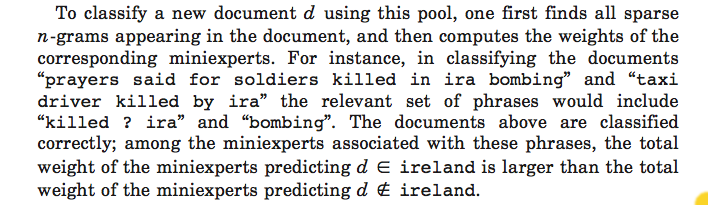
\includegraphics[height=3cm]{figures/TextClassification1.png}
\end{center}
\end{frame}

\begin{frame}
\frametitle{Using Specialists for text classification}
\begin{center}
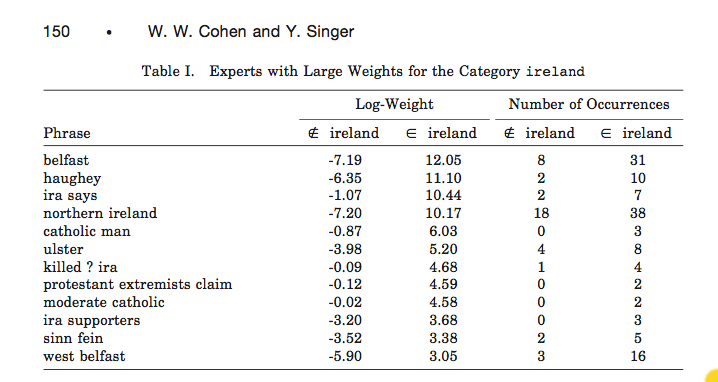
\includegraphics[height=6cm]{figures/TextClassification2.png}
\end{center}
\end{frame}

\section{Tracking}
\begin{frame}
\frametitle{Dynamics using Kalman Filters}
Too many resources to list.
\begin{center}
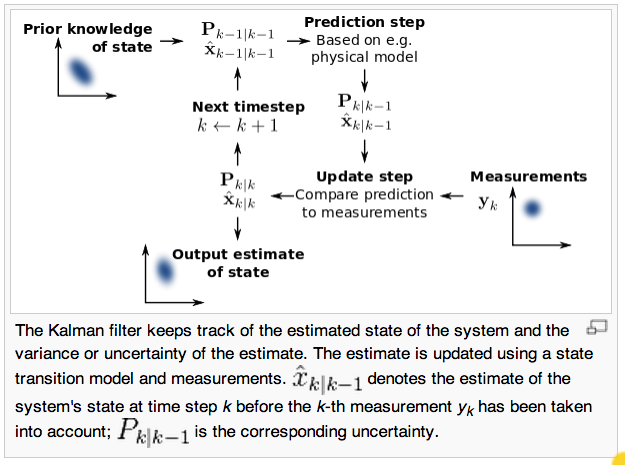
\includegraphics[height=6cm]{figures/KalmanFilter.png}
\end{center}
\end{frame}

\begin{frame}
\frametitle{Dynamics using Particle Filters}
{\bf The unscented particle filter} / R. Van Der Merwe, A. Doucet, N. De Freitas, E. Wan
\begin{center}
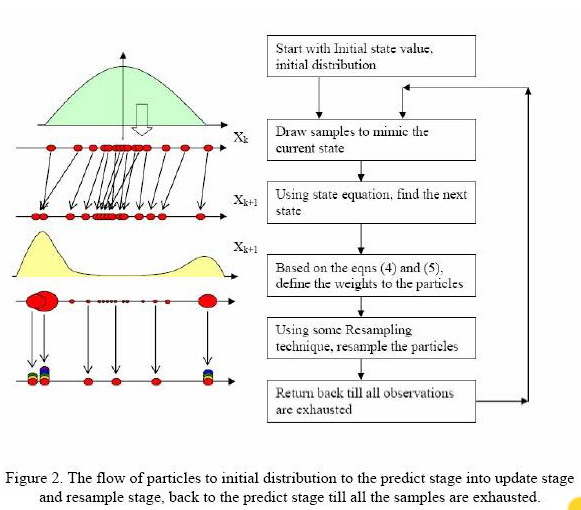
\includegraphics[height=6cm]{figures/ParticleFilters.png}
\end{center}
\end{frame}

\begin{frame}
\frametitle{Specialists for dynamics}
\begin{itemize}
\item Tracking for interaction.
\item Handwriting recognition (Sunsern)
\end{itemize}
\end{frame}

\begin{frame}
\frametitle{Experts for appearance modeling}
\begin{itemize}
\item Templates - sample image patch and compare to future patches.
\item Identify location of object using a boosted combination of
  low-level features. (Online Boosting)
\item Specialists: tracking the best appearance model.
\item Within a small set: assuming that old appearances will recur.
\end{itemize}
\end{frame}

\begin{frame}
\frametitle{Confidence}
\begin{itemize}
\item Can we quantify the confidence we have in our prediction?
\item If there is a set of awake specialists that have a large weight
  and make similar predictions.
\item In Kalman filters: covariance of the posterior distribution.
\end{itemize}
\end{frame}

\begin{frame}
\frametitle{Co-Training}
\begin{itemize}
\item When tracking, we have no ground truth - how can we train our
  models?
\item Co-training: Train in proportion to confidence
\item When Dynamics is confident: use it to train appearance.
\item When appearance is confident: use it to train dynamics.
\item Specialists can correspond to using different features,
  different image resolutions etc.
\end{itemize}
\end{frame}

\iffalse
\fi
\end{document}


